% **** Szablon pracy magisterskiej, licencjackiej lub inżynierskiej ****

\documentclass[polish,12pt,twoside,a4paper]{report}



% *************** Definicje stylu dokumentu ***************

% *********************************************************************************
% W pliku tym zdefiniowany jest wygl¹d dokumentu.
% Zmiany tutaj nie s¹ konieczne o ile nie zamierzasz zmieniaæ wygl¹du dokumentu.
% *********************************************************************************

% *************** Za³adowanie pakietów ***************
\usepackage[a4paper,twoside,left=2.0cm,right=1.5cm,top=1.5cm,bottom=1.5cm]{geometry}
\usepackage[T1]{fontenc}
%\usepackage[cp1250]{inputenc}
\usepackage[utf8]{inputenc}
\usepackage[polish]{babel}
\usepackage{amsmath}
\usepackage{amsfonts}
\usepackage{graphicx}
\usepackage{graphics}
\usepackage{float}
\usepackage{times}
\usepackage{indentfirst}%wciecia a nowych akapitach
\usepackage{listings}
\usepackage{url}
\usepackage[colorlinks=true, linkcolor=black, urlcolor=black, citecolor=black]{hyperref}

\selectlanguage{polish}

%szerokoœœ wciêæ
\setlength{\parindent}{1.25cm}

%numeracja stron
\usepackage{fancyhdr}
\pagestyle{fancy}
\fancyhf{} % usun biezace ustawienia pagin
\fancyhead[LE,RO]{ }
\fancyhead[LO]{ }
\fancyhead[RE]{ }
\fancyfoot[LE,RO]{\small\thepage}
\fancyfoot[LO]{ }
\fancyfoot[RE]{ }
\renewcommand{\headrulewidth}{0.0pt}
\renewcommand{\footrulewidth}{0.0pt}
\addtolength{\headheight}{0.0pt} % pionowy odstep na kreske
\fancypagestyle{plain}{%
\fancyhead{} % usun p. górne na stronach pozbawionych
% numeracji (plain)
\renewcommand{\headrulewidth}{0.0pt} % pozioma kreska
}

% *************** Definicje niektórych kolorów ***************
\usepackage{color}

\definecolor{greenyellow}   {cmyk}{0.15, 0   , 0.69, 0   }
\definecolor{yellow}        {cmyk}{0   , 0   , 1   , 0   }
\definecolor{goldenrod}     {cmyk}{0   , 0.10, 0.84, 0   }
\definecolor{dandelion}     {cmyk}{0   , 0.29, 0.84, 0   }
\definecolor{apricot}       {cmyk}{0   , 0.32, 0.52, 0   }
\definecolor{peach}         {cmyk}{0   , 0.50, 0.70, 0   }
\definecolor{melon}         {cmyk}{0   , 0.46, 0.50, 0   }
\definecolor{yelloworange}  {cmyk}{0   , 0.42, 1   , 0   }
\definecolor{orange}        {cmyk}{0   , 0.61, 0.87, 0   }
\definecolor{burntorange}   {cmyk}{0   , 0.51, 1   , 0   }
\definecolor{bittersweet}   {cmyk}{0   , 0.75, 1   , 0.24}
\definecolor{redorange}     {cmyk}{0   , 0.77, 0.87, 0   }
\definecolor{mahogany}      {cmyk}{0   , 0.85, 0.87, 0.35}
\definecolor{maroon}        {cmyk}{0   , 0.87, 0.68, 0.32}
\definecolor{brickred}      {cmyk}{0   , 0.89, 0.94, 0.28}
\definecolor{red}           {cmyk}{0   , 1   , 1   , 0   }
\definecolor{orangered}     {cmyk}{0   , 1   , 0.50, 0   }
\definecolor{rubinered}     {cmyk}{0   , 1   , 0.13, 0   }
\definecolor{wildstrawberry}{cmyk}{0   , 0.96, 0.39, 0   }
\definecolor{salmon}        {cmyk}{0   , 0.53, 0.38, 0   }
\definecolor{carnationpink} {cmyk}{0   , 0.63, 0   , 0   }
\definecolor{magenta}       {cmyk}{0   , 1   , 0   , 0   }
\definecolor{violetred}     {cmyk}{0   , 0.81, 0   , 0   }
\definecolor{rhodamine}     {cmyk}{0   , 0.82, 0   , 0   }
\definecolor{mulberry}      {cmyk}{0.34, 0.90, 0   , 0.02}
\definecolor{redviolet}     {cmyk}{0.07, 0.90, 0   , 0.34}
\definecolor{fuchsia}       {cmyk}{0.47, 0.91, 0   , 0.08}
\definecolor{lavender}      {cmyk}{0   , 0.48, 0   , 0   }
\definecolor{thistle}       {cmyk}{0.12, 0.59, 0   , 0   }
\definecolor{orchid}        {cmyk}{0.32, 0.64, 0   , 0   }
\definecolor{darkorchid}    {cmyk}{0.40, 0.80, 0.20, 0   }
\definecolor{purple}        {cmyk}{0.45, 0.86, 0   , 0   }
\definecolor{plum}          {cmyk}{0.50, 1   , 0   , 0   }
\definecolor{violet}        {cmyk}{0.79, 0.88, 0   , 0   }
\definecolor{royalpurple}   {cmyk}{0.75, 0.90, 0   , 0   }
\definecolor{blueviolet}    {cmyk}{0.86, 0.91, 0   , 0.04}
\definecolor{periwinkle}    {cmyk}{0.57, 0.55, 0   , 0   }
\definecolor{cadetblue}     {cmyk}{0.62, 0.57, 0.23, 0   }
\definecolor{cornflowerblue}{cmyk}{0.65, 0.13, 0   , 0   }
\definecolor{midnightblue}  {cmyk}{0.98, 0.13, 0   , 0.43}
\definecolor{navyblue}      {cmyk}{0.94, 0.54, 0   , 0   }
\definecolor{royalblue}     {cmyk}{1   , 0.50, 0   , 0   }
\definecolor{blue}          {cmyk}{1   , 1   , 0   , 0   }
\definecolor{cerulean}      {cmyk}{0.94, 0.11, 0   , 0   }
\definecolor{cyan}          {cmyk}{1   , 0   , 0   , 0   }
\definecolor{processblue}   {cmyk}{0.96, 0   , 0   , 0   }
\definecolor{skyblue}       {cmyk}{0.62, 0   , 0.12, 0   }
\definecolor{turquoise}     {cmyk}{0.85, 0   , 0.20, 0   }
\definecolor{tealblue}      {cmyk}{0.86, 0   , 0.34, 0.02}
\definecolor{aquamarine}    {cmyk}{0.82, 0   , 0.30, 0   }
\definecolor{bluegreen}     {cmyk}{0.85, 0   , 0.33, 0   }
\definecolor{emerald}       {cmyk}{1   , 0   , 0.50, 0   }
\definecolor{junglegreen}   {cmyk}{0.99, 0   , 0.52, 0   }
\definecolor{seagreen}      {cmyk}{0.69, 0   , 0.50, 0   }
\definecolor{green}         {cmyk}{1   , 0   , 1   , 0   }
\definecolor{forestgreen}   {cmyk}{0.91, 0   , 0.88, 0.12}
\definecolor{pinegreen}     {cmyk}{0.92, 0   , 0.59, 0.25}
\definecolor{limegreen}     {cmyk}{0.50, 0   , 1   , 0   }
\definecolor{yellowgreen}   {cmyk}{0.44, 0   , 0.74, 0   }
\definecolor{springgreen}   {cmyk}{0.26, 0   , 0.76, 0   }
\definecolor{olivegreen}    {cmyk}{0.64, 0   , 0.95, 0.40}
\definecolor{rawsienna}     {cmyk}{0   , 0.72, 1   , 0.45}
\definecolor{sepia}         {cmyk}{0   , 0.83, 1   , 0.70}
\definecolor{brown}         {cmyk}{0   , 0.81, 1   , 0.60}
\definecolor{tan}           {cmyk}{0.14, 0.42, 0.56, 0   }
\definecolor{gray}          {cmyk}{0   , 0   , 0   , 0.50}
\definecolor{black}         {cmyk}{0   , 0   , 0   , 1   }
\definecolor{white}         {cmyk}{0   , 0   , 0   , 0   } 

% *************** Koniec definicji stylu dokumentu ***************


%definicja przydatnych poleceń
\newcommand{\wydzial}{KOLEGIUM INFORMATYKI STOSOWANEJ}
\newcommand{\kierunek}{Kierunek: INFORMATYKA}
\newcommand{\specjalnosc}{Specjalność: {Inżynieria Danych (ID)}}
\newcommand{\autor}{Casper Czech}
\newcommand{\album}{Nr albumu studenta w71019}
\newcommand{\temat}{System obsługi parkingu}
\newcommand{\promotor}{mgr inż. Ewa Żesławska}
\newcommand{\typpracy}{Praca projektowa programowanie obiekotwe C\#}
\newcommand{\miasto}{Rzeszów}
\newcommand{\rok}{2025}

\begin{document}

% *************** Włączenie definicji pierwszych stron ***************
% *************** Strony tytułowe ***************

% ************************************************************
% W tym miejscu znajduje sie definicja wyglądu pierwszych stron:
% strony tytułowej, strony z oświadczeniem o treści pracy
% i strony ze spisem treści
% ************************************************************
% *************** Strona tytułowa ***************
%umieszczenie logo i nazwy uczelni
\noindent
\parbox{65mm}{
\includegraphics[width=13.0cm, height=3.0cm]{logoWSIiZ}}

\vspace{10mm}
\begin{center}
{\Large{}\textbf{\wydzial}}
\end{center}
\vspace{10mm}
\noindent
\hspace{30mm}{\Large{}\textbf{\kierunek}}\\

\noindent
\hspace{30mm}{\Large{}\textbf{\specjalnosc}}
\vspace{30mm}
\begin{center}
	{\large{}\autor}\\
	{\large{}\album}\\
	\vspace{15pt}
	{\huge{}\textbf{\textit{\temat}}}\\
	\vspace{20pt}
	{\normalsize{}Prowadzący: \promotor}\\
	\vspace{100pt}
	{\LARGE{}\textbf{\typpracy}}\\
	\vspace{190pt}
	{\large{}\textbf{\miasto {} \rok}}
\end{center}

% pusta zawartość stopki - brak numeru strony
\thispagestyle{empty}

% *************** Strona z oświadczeniem o treści pracy ***************
\newpage
\text{}

\thispagestyle{empty}
\newpage


% *************** Spis treści ***************
\tableofcontents
% pusta zawartość stopki - brak numeru strony
\thispagestyle{empty}
\newpage

% *************** Koniec pliku front.tex ***************



% *************** Część główna pracy ***************
\chapter*{Wstęp}

System obsługi parkingu to aplikacja umożliwiająca zarządzanie przestrzenią parkingową w sposób zautomatyzowany. System pozwala na rejestrowanie przyjazdów i odjazdów pojazdów, kontrolę zajętości miejsc oraz wizualizację stanu parkingu. Dzięki temu zapewnia przejrzystość w użytkowaniu parkingu oraz umożliwia szybkie wyszukiwanie informacji o pojazdach na podstawie numeru rejestracyjnego lub innych kryteriów.

Aplikacja obsługuje różne rodzaje pojazdów, takie jak motocykle, samochody osobowe i autobusy, które zajmują różną ilość miejsc na parkingu. Każdy pojazd posiada przypisane współrzędne zajmowanych pól oraz numer rejestracyjny. System rejestruje także historię zdarzeń, takich jak przyjazdy i odjazdy, co pozwala na późniejszą analizę ruchu na parkingu.

\
\addcontentsline{toc}{chapter}{Wstęp}
\newpage
% ********** Rozdział 1 **********
\chapter{Opis założeń projektu}
\section{Cele projetu}
%\subsection{Tytuł pierwszego podpunktu}

Celem projektu jest stworzenie systemu zarządzania parkingiem, który umożliwi efektywne monitorowanie i kontrolowanie zajętości miejsc parkingowych w zorganizowany sposób. System ma zapewniać:
Automatyzację procesów:
Obsługa przyjazdów i odjazdów pojazdów.
Automatyczna weryfikacja dostępności miejsc parkingowych w zależności od wymagań przestrzennych różnych typów pojazdów.
Wizualizację stanu parkingu:
Czytelna i intuicyjna reprezentacja graficzna zajętości parkingu w konsoli za pomocą znaków tekstowych.
Rejestrację zdarzeń:
Przechowywanie informacji o każdym zdarzeniu, takim jak przyjazdy i odjazdy pojazdów, wraz z datą i godziną.
Możliwość przeszukiwania historii na podstawie numeru rejestracyjnego pojazdu lub zakresu czasowego.
Wsparcie dla różnych typów pojazdów:
Obsługa motocykli, samochodów osobowych oraz autobusów, z uwzględnieniem różnej liczby miejsc zajmowanych przez te pojazdy.
Ułatwienie zarządzania przestrzenią parkingową:
Zwiększenie przejrzystości stanu zajętości miejsc.
Szybkie znajdowanie informacji o pojazdach zaparkowanych lub już odjeżdżających.
Dzięki wdrożeniu tego systemu możliwe jest zwiększenie wydajności operacyjnej parkingu, zminimalizowanie błędów w alokacji miejsc oraz ułatwienie pracy personelu zarządzającego parkingiem. System jest również skalowalny i może zostać zaadaptowany do różnej wielkości parkingów oraz dodatkowych wymagań użytkowników.

\end{itemize}


\section{Wymagania funkcjonale i niefunkcjonalne}

\noindent \textbf{Wymagania funkcjonalne}
\begin{itemize}
    \item Wymagania funkcjonalne
Zarządzanie pojazdami:

\item Możliwość dodawania pojazdu na parking z określeniem numeru rejestracyjnego oraz wymagań przestrzennych (typ pojazdu).
\item Usuwanie pojazdu z parkingu na podstawie numeru rejestracyjnego.
\item Walidacja dostępności miejsca:

\item Weryfikacja, czy wskazane miejsce parkingowe jest dostępne dla danego typu pojazdu.
\item Blokada dodawania pojazdu, jeśli miejsca są zajęte lub wykraczają poza granice parkingu.
\item Wizualizacja parkingu:

\item Wyświetlanie aktualnego stanu parkingu w konsoli w formie graficznej (np. znaki tekstowe reprezentujące zajętość miejsc: M dla motocykli, C dla samochodów, B dla autobusów).
Historia zdarzeń:

\item Rejestrowanie informacji o każdym przyjeździe i odjeździe pojazdu, w tym numeru rejestracyjnego, typu pojazdu, zajętych miejsc oraz daty i godziny zdarzenia.
Wyszukiwanie pojazdów i zdarzeń:

Możliwość wyszukiwania informacji o pojazdach w historii zdarzeń na podstawie:
Numeru rejestracyjnego.
Daty i godziny przyjazdu lub odjazdu.

\end{itemize}

\noindent \textbf{Wymagania niefunkcjonalne }
\begin{itemize}

\item System powinien działać płynnie przy obsłudze parkingów o różnej wielkości (od kilkunastu do kilkuset miejsc).

\item Skalowalność:
Projekt powinien umożliwiać łatwe dostosowanie do większych parkingów lub nowych typów pojazdów.
Czytelność interfejsu:

\item Wizualizacja parkingu powinna być czytelna i intuicyjna dla użytkownika, umożliwiając szybkie zrozumienie aktualnego stanu zajętości miejsc.
Niezawodność:

\item System powinien zapobiegać błędom, takim jak umieszczanie dwóch pojazdów na tym samym miejscu lub dodawanie pojazdu poza granice parkingu.
Przechowywanie danych:

\item Historia zdarzeń powinna być przechowywana w sposób trwały (np. w pamięci programu podczas działania lub w pliku).
Łatwość rozbudowy:

\item Kod powinien być modularny i dobrze udokumentowany, aby umożliwić łatwe dodawanie nowych funkcjonalności lub modyfikację istniejących.
Użyteczność:

\item System powinien być prosty w obsłudze, zarówno dla operatorów, jak i dla osób zarządzających parkingiem.
Bezpieczeństwo danych:

\item Numer rejestracyjny i inne informacje powinny być przechowywane w sposób bezpieczny, zgodnie z wymogami ochrony danych (np. w kontekście RODO, jeśli dotyczy).

\end{itemize}
 




% ********** Koniec rozdziału **********

\newpage
% ********** Rozdział 2 **********
\chapter{Opis struktury projektu}
\section{Podstawowe informacje techniczne}
Aplikacja została napisana w języku C\# i uruchamiana jest w konsoli.

\section{Minimalne wymagania sprzętowe}
\begin{itemize}
    \item Procesor minimum 2 GHz.
    \item 2 GB pamięci RAM.
    \item System operacyjny Windows/Linux.
    \item Zainstalowane środowisko .NET.
\end{itemize}

\section{Hierarchia klas}

System składa się z hierarchii klas, które reprezentują różne typy pojazdów oraz logikę zarządzania parkingiem. 
Podstawową klasą jest \textbf{Pojazd}, która jest klasą abstrakcyjną i stanowi bazę dla klas: \textbf{Motocykl}, \textbf{Samochod} oraz \textbf{Autobus}. 
Klasa \textbf{Parking} odpowiada za zarządzanie pojazdami i przechowywanie ich stanu. 
Program steruje aplikacją i zapewnia interakcję z użytkownikiem.

\section{Diagram klas}

Poniżej przedstawiono diagram klas UML obrazujący relacje między klasami w systemie:

\begin{itemize}
    \item \textbf{Program} – klasa główna, odpowiedzialna za uruchomienie aplikacji i zarządzanie logiką programu.
    \item \textbf{Parking} – klasa zarządzająca stanem parkingu, przechowująca informacje o zajętych miejscach oraz umożliwiająca dodawanie i usuwanie pojazdów.
    \item \textbf{Pojazd} – klasa bazowa dla różnych typów pojazdów, przechowuje informacje o numerze rejestracyjnym, typie pojazdu oraz zajmowanych miejscach parkingowych.
    \begin{itemize}
        \item \textbf{Motocykl} – klasa dziedzicząca po klasie Pojazd, reprezentująca motocykl na parkingu.
        \item \textbf{Samochód} – klasa dziedzicząca po klasie Pojazd, reprezentująca standardowy samochód osobowy.
        \item \textbf{Autobus} – klasa dziedzicząca po klasie Pojazd, zajmująca większą liczbę miejsc na parkingu.
    \end{itemize}
\end{itemize}

\subsection{Schemat klas}
Powyżej przedstawiony jest diagram klas obrazujący zależności między poszczególnymi elementami systemu.

\begin{figure}[]
    \centering
    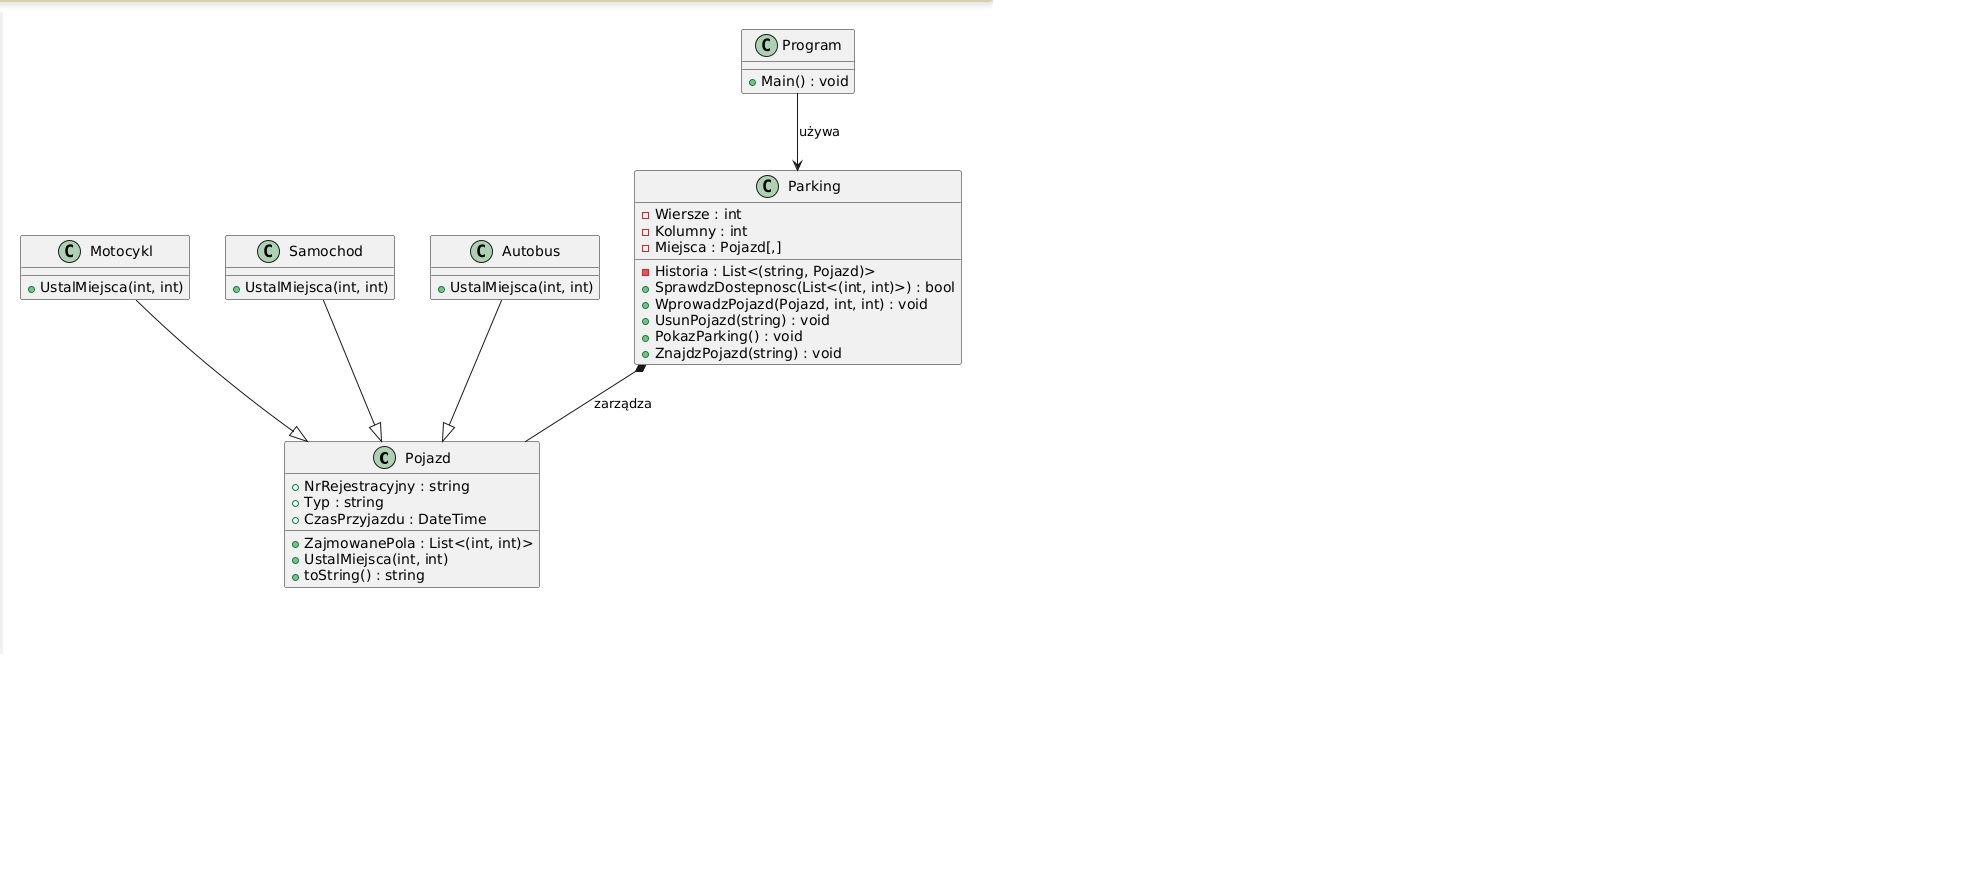
\includegraphics[width=\textwidth]{diagram_klas2.jpg}
    \caption{Diagram klas systemu parkingowego}
    \label{fig:diagram_klas}
\end{figure}






% ********** Koniec rozdziału **********

\newpage
% ********** Rozdział 3 **********
\chapter{Harmonogram realizacji projektu}

\section{Harmonogram}
\begin{figure}[ht]
    \centering
    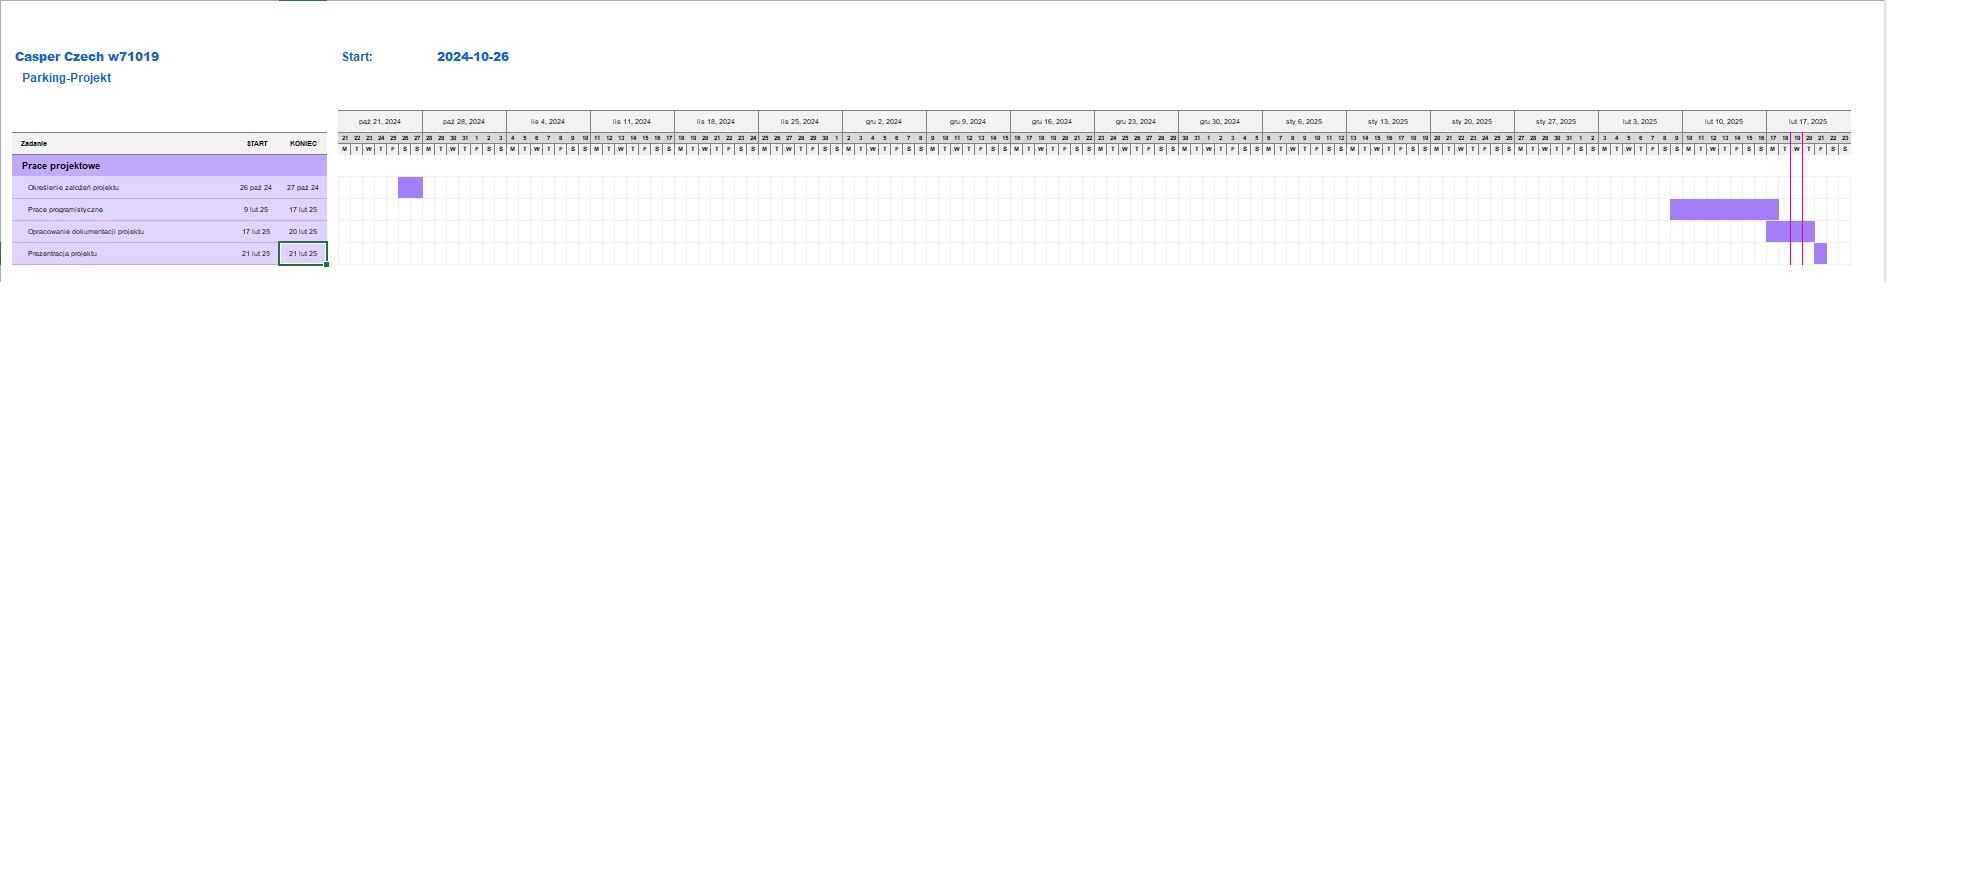
\includegraphics[width=1\linewidth]{harmonogram.jpg}
    \caption{Diagram Gantta}
\end{figure}
Realizacja projektu, przedstawiona na powyższym diagramie Gantta, obejmowała następujące etapy:
\begin{itemize}
    \item określenie założeń projektu - 26-27.10.2024,
    \item prace programistyczne - 07-17.02.2025,
    \item opracowanie dokumentacji projektu - 17-20.02.2025,
    \item prezentację i obronę projektu - 21.02.2025.
\end{itemize}

\section{Repozytorium i system kontroli wersji}
Kod projektu został przygotowany przy użyciu systemu kontroli wersji Git, a hostowany jest na platformie GitHub.
Repozytorium jest dostępne pod adresem: \url{https://github.com/3Czester/Programowanie_Casper_Czech_w71019}.


% ********** Koniec rozdziału **********
\newpage
% ********** Rozdział 4 **********
\chapter{Prezentacja warstwy użytkowej projektu}

Aplikacja do zarządzania parkingiem pozwala na wykonywanie operacji związanych z dodawaniem, usuwaniem oraz wyszukiwaniem pojazdów, a także wizualizację stanu parkingu. Poniżej przedstawiono zrzuty ekranu wraz z opisem poszczególnych funkcjonalności.

\section{Dodawanie pojazdu}
Dodanie pojazdu do systemu odbywa się poprzez podanie jego danych, takich jak numer rejestracyjny, typ pojazdu oraz miejsce parkingowe. Na poniższym zrzucie ekranu przedstawiono interfejs umożliwiający dodanie pojazdu.
\begin{figure}[H]
    \centering
    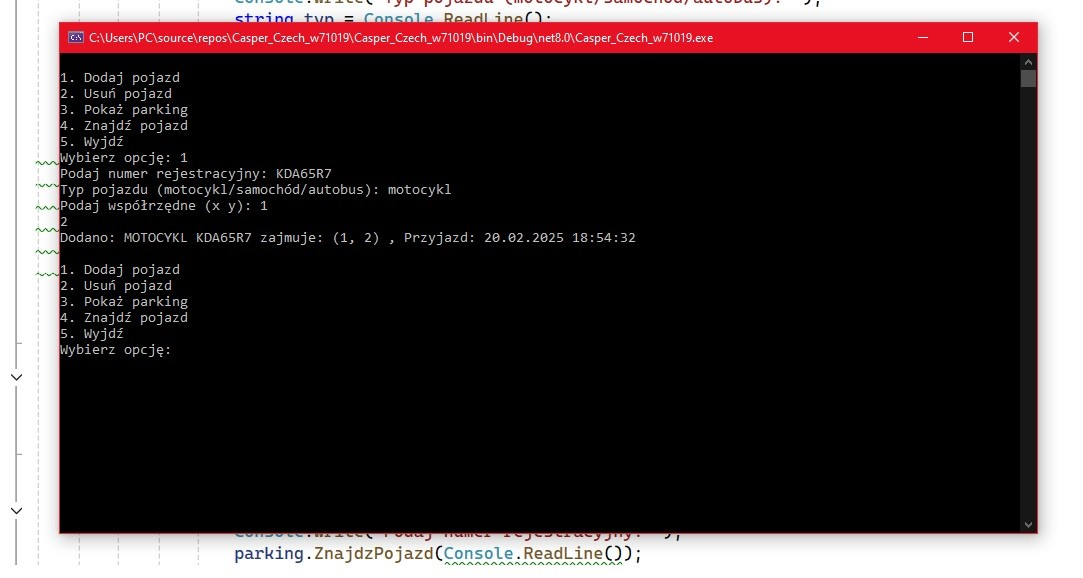
\includegraphics[width=0.8\linewidth]{Dodaj_pojazd.jpg}
    \caption{Dodawanie pojazdu do systemu}
    \label{fig:enter-label}
\end{figure}

\section{Wyświetlanie stanu parkingu}
Aplikacja umożliwia wizualizację aktualnego stanu parkingu, przedstawiając zajęte i wolne miejsca. Użytkownik może w łatwy sposób sprawdzić, które miejsca są dostępne.


\begin{figure}[H]
    \centering
    \includegraphics[width=0.8\linewidth]{Pokaż_parking.jpg}
    \caption{Widok parkingu w systemie}
    \label{fig:enter-label}
\end{figure}
\section{Usuwanie pojazdu}
Gdy pojazd opuszcza parking, użytkownik może usunąć go z systemu, co automatycznie zwalnia zajmowane miejsce.

\begin{figure}[H]
    \centering
    \includegraphics[width=0.8\linewidth]{Usuń_pojazd.jpg}
    \caption{Usuwanie pojazdu z systemu}
\end{figure}

\section{Wyszukiwanie pojazdu}
W celu szybkiego odnalezienia pojazdu system umożliwia jego wyszukiwanie po numerze rejestracyjnym. 

\begin{figure}[H]
    \centering
    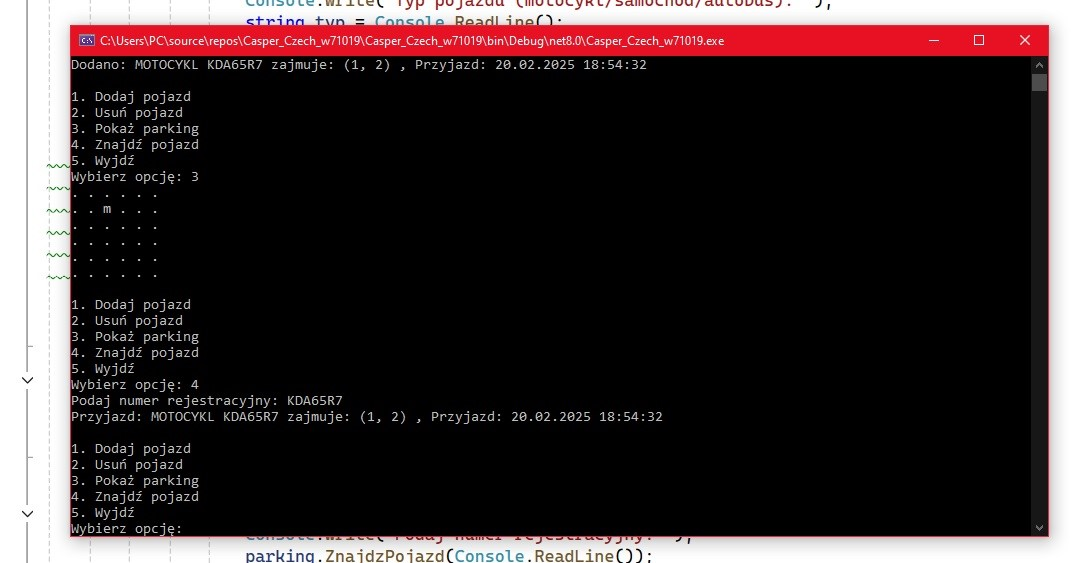
\includegraphics[width=0.8\linewidth]{Znajdz_pojazd.jpg}
    \caption{Wyszukiwanie pojazdu}
\end{figure}

\section{Zamykanie aplikacji}
Użytkownik ma możliwość zamknięcia aplikacji poprzez odpowiednią opcję w menu.

\begin{figure}[H]
    \centering
    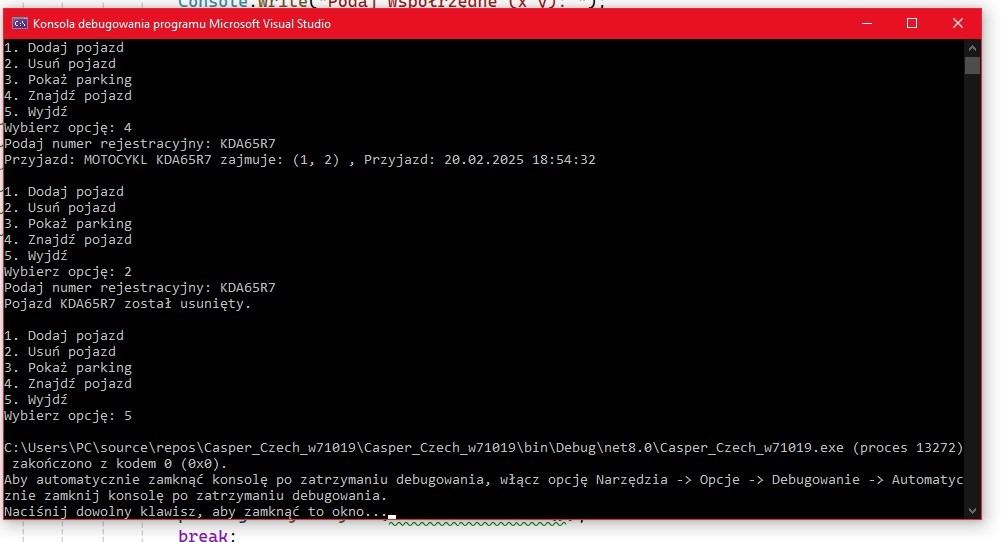
\includegraphics[width=0.8\linewidth]{Wyjdz.jpg}
    \caption{Zamykanie aplikacji}
\end{figure}





% ********** Koniec rozdziału **********

\newpage
% ********** Rozdział 5 **********
\chapter{Podsumowanie}

W ramach projektu wykonałem aplikację konsolową do zarządzania systemem parkingowym, wykorzystując język C\# oraz technologię .NET.

Realizacja projektu obejmowała następujące zadania:
\begin{itemize}
    \item określenie założeń funkcjonalnych i niefunkcjonalnych,
    \item implementację kluczowych funkcjonalności aplikacji, w tym:
    \begin{itemize}
        \item obsługę różnych typów pojazdów i ich miejsc parkingowych,
        \item wizualizację stanu parkingu w konsoli,
        \item rejestrowanie przyjazdów i odjazdów pojazdów,
    \end{itemize}
    \item stworzenie dokumentacji projektowej,
    \item prezentację i obronę projektu.
\end{itemize}

W ramach dalszego rozwoju planuję dodać następujące funkcjonalności usprawniające działanie aplikacji:
\begin{itemize}
    \item rozszerzenie obsługi o więcej typów pojazdów,
    \item integrację z bazą danych w celu trwałego przechowywania informacji o miejscach parkingowych,
    \item dodanie interfejsu graficznego w celu lepszego zobrazowania zajętych miejsc,
    \item wprowadzenie mechanizmu rezerwacji miejsc parkingowych.
\end{itemize}




% ********** Koniec rozdziału **********


\newpage
\input{R6.tex}
\newpage

% *************** Bibliografia ***************
\begin{thebibliography}{9}
\addcontentsline{toc}{chapter}{Bibliografia}

\bibitem{csharp_podstawy} Piotr Wróblewski, {\it C# 10.0. Wprowadzenie do programowania}, Wydawnictwo Helion, Gliwice 2022.  
\bibitem{csharp_zaawansowane} Krzysztof Foltak, {\it C#. Praktyczny kurs. Wydanie IV}, Wydawnictwo Helion, Gliwice 2021.  
\bibitem{csharp_wzorce} Leszek Grzesiak, {\it Wzorce projektowe w C#}, Wydawnictwo Helion, Gliwice 2020.  
\bibitem{programowanie_obiektowe} Grzegorz Dunikowski, {\it Programowanie obiektowe w języku C#}, Wydawnictwo Helion, Gliwice 2019.  
\bibitem{bazy_danych} Marek Konieczny, {\it Bazy danych i ich integracja z C#}, Wydawnictwo Helion, Gliwice 2021.  
\bibitem{git} Rafał Kuć, {\it Git. Rozproszony system kontroli wersji}, Wydawnictwo Helion, Gliwice 2020.  
\bibitem{zarzadzanie_projektami} Roman Kotapski, {\it Zarządzanie projektami. Metody, narzędzia, techniki}, Wydawnictwo PWE, Warszawa 2018.  
\bibitem{smart_parking} Tomasz Górski, {\it Inteligentne systemy transportowe}, Wydawnictwo Naukowe PWN, Warszawa 2022.  

\end{thebibliography}
\newpage


% *************** Zakończenie ***************
\chapter{Literatura}
\begin{itemize}
    \item Dokumentacja języka C\# - \url{https://learn.microsoft.com/en-us/dotnet/csharp/}
    \item Dokumentacja .NET - \url{https://dotnet.microsoft.com/}
\end{itemize}

\end{document}
% *************** Koniec pliku szablon.tex ***************
